\chapter{Rules Overview}\label{chap:rules_overview}

\begin{figure}[!htb]
\centering
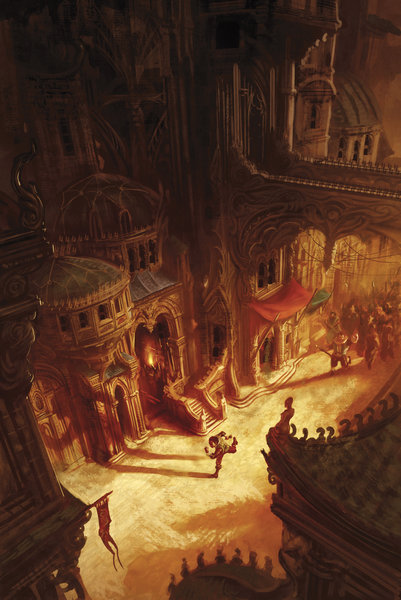
\includegraphics[width=0.5\linewidth]{images/runner.jpg}
\end{figure}

\begin{centering}
    \textit{This is a very rough summary of the Core Rules. Refer to the Genesys Core Rulebook for the full Rules.}
\end{centering}

\begin{table*}[!htb]
\begin{GenesysTable}{Maneuvers}{maneuvers}{ =l +X}
Maneuver                &   Description\\
Aim                     &   Gain \boost on next combat check, or gain \boost\boost on next combat check if aiming for 2 consecutive maneuvers.\\
Aim (Called Shot)       &   Gain \setback\setback on next combat check, or gain \setback on next combat check if aiming for 2 consecutive maneuvers.\\
Assist                  &   Engaged ally adds \boost to their next check, Can stack from other assists.\\
Guarded Stance          &   Gain melee defense 1. Add \setback to combat checks, until end of the next turn.\\
Interact w. Enviroment  &   Move a large item, open/close door, press button, pick up weapon, etc.\\
Taking Cover            &   Gain ranged defense 1. Opponents add \setback to skill checks (e.g Perception), or \setback\setback if particularly well-covered.\\
Manage Gear             &   Draw, holster, ready or load a weapon. Retrieve/put away stored item.\\
Mount/Dismount          &   A domestic animal, vehicle, cockpit, gunnery station etc.\\
Direct Mount            &   Mount moves 2 maneuvers.\\
Move                    &   Change range increment or Engage/disengage from melee. Difficult Terrain doubles the amount of maneuvers required.\newline
                            Engaged $\Rightarrow$ 1 $\Rightarrow$ Short $\Rightarrow$ 1 $\Rightarrow$ Medium $\Rightarrow$ 2 $\Rightarrow$ Long $\Rightarrow$ 2 $\Rightarrow$ Extreme.\\
Drop Prone / Stand up   &   While you are prone, add \setback to all ranged attacks targeting you and add \boost to all melee attacks made against you.\\
Preparation             &   Some actions require additional preparation to perform effecively.\\
\end{GenesysTable}
\end{table*}

\begin{multicols}{2}

\subsection{Turns}
\subsubsection{Manouvers}
Maneuvers are activities that aren’t complex enough to
warrant a skill check, but still involve time and effort
on the part of a character.

To perform a second maneuver the character must spend either:
\begin{description}
    \item An action.
    \item Two strain.
    \item \advantage\advantage generated on a skill check.
\end{description}

Characters may not perform more than two maneuvers during their turn.
The following are some examples of maneuvers:

\FloatBarrier

\subsubsection{Actions}
Actions are important activities that are vital to a character's accomplishment
of a goal. Each character may normally only perform one action during their
turn, likely the most important activity they undertake during their turn.
Actions almost always involve performing a skill check, although certain
character abilities may require using an action to activate them.

The following are some examples of actions:
\begin{description}
    \item Unlocking a locked door.
    \item Shooting a bow
    \item Punching or grappling an opponent.
    \item Instructing allies with a series of orders.
    \item Performing first aid on an ally.
    \item Sneaking up on a vigilant foe.
    \item Climbing a cliff.
\end{description}
Out of all of these options, the most common during combat are those that
involve attacking an opponent. Attacking an opponent requires a combat
skill check, sometimes referred to in shorthand as a combat check or
simply an attack.

\subsection{Performing a Combat Check}
\begin{table}[H]
\begin{GenesysTable}{Ranged Attack Difficulties}{attack-ranged-difficulties}{ =l +X}
Range Band  & Difficulty\\
Engaged     & \textbf{Easy} (\difficulty) plus modifiers depending of the weapon used.\\
Short       & \textbf{Easy} (\difficulty)\\
Medium      & \textbf{Average} (\difficulty\difficulty)\\
Long        & \textbf{Hard }(\difficulty\difficulty\difficulty)\\
Extreme     & \textbf{Daunting }(\difficulty\difficulty\difficulty\difficulty)\\
\end{GenesysTable}
\end{table}

\subsubsection{Spending Dice in Combat}
\begin{table*}[!htb]
\begin{GenesysTable}{Spending Advantage and Triumph in Combat}{combat-advantage}{ =l +X}
Cost        & Result Option\\
\advantage or \triumph  & Recover 1 strain.\newline
                          Add \boost to the next allied character's check\newline
                          Notice a single important point in the ongoing conflict, such as a weakspot in the armour.\newline
                          Inflict a Critical Injury with a successful attack that deals damage poast soak (\advantage cost may vary).\newline
                          Activate an item quality (\advantage cost may vary).\\
\advantage\advantage or \triumph  & Perform an immediate free maneuver that does not exceed the limit of two maneuvers per turn.\newline
                                    Add \setback to the targeted character's next check.\newline
                                    Add \boost to any allied character's next check, including that of the active character.\\
\advantage\advantage\advantage or \triumph  & Negate the targeted enemy's defense (such as the defense gained from cover, equipment, or performing the guarded stance
                                              maneuver) until the end of the current round.\newline
                                              Ignore penalizing environmental effects such as inclement weather, zero gravity, or similar circumstances until the end of the
                                              active character’s next turn.\newline
                                              When dealing damage to a target, have the attack disable the opponent or one piece of gear rather than dealing wounds or strain.\newline
                                              This could include hobbling them temporarily with a shot to the legThis should be agreed upon by the
                                              player and the GM, and the effects are up to the GM. The effects should be temporary and not too excessive.\newline
                                              Gain +1 melee or ranged defense until the end of the active character's next turn.\newline
                                              Force the target to drop a melee or ranged weapon they are wielding.\\
\triumph  &         Upgrade the difficulty of the targeted character’s next check.\newline
                    Upgrade the ability of any allied character’s next check, including that of the current active character.\newline
                    Do something vital, such as shooting the controls to the nearby blast doors to seal them shut.\newline
                    On an Initiative check, perform an immediate free maneuver before combat begins.\\
\triumph\triumph  & When dealing damage to a target, have the attack destroy a
                    piece of equipment the target is using, such as blowing up
                    their assault rifle or slicing their sword in half. \\
\end{GenesysTable}
\begin{GenesysTable}{Spending Threat and Despair in Combat}{combat-threat}{ =l +X}
Cost        & Result Option\\
\setback or \despair  & The active character suffers 1 strain.\newline
                          The active character loses the benefits of a prior maneuver (such as from taking cover or assuming a guarded stance) until they perform the maneuver again.\\
\setback\setback or \despair  & An opponent may immediately perform one free maneuver as an incidental in response to the active character's check.\newline
                                    Add \boost to the targeted character's next check.\newline
                                    The active character or an allied character suffers \boost on their next action.\\
\setback\setback\setback or \despair  & The active character falls prone.\newline
                                              The active character grants the enemy a significant advantage in the ongoing
                                              encounter, such as accidentally blasting the controls to a bridge the active
                                              character was planning to use for their escape.\\
\despair  & Upgrade the difficulty of an allied character's next check or the next check of the current active character.\newline
            The tool, Brawl, or Melee weapon the character is using becomes damaged.\\
\despair\despair  & The character's weapon immediately breaks if it has the \iqtyref{fragile} Quality.\\
\end{GenesysTable}
\end{table*}

\end{multicols}

\FloatBarrier

\section{Injury}
\subsection{Critical hits}

\begin{table*}[!htb]
\begin{GenesysTable}{Critical Hits}{critical-hits}{ =l +l +X}
D100    & Severity              & Result\\
01-05   & \textbf{Easy} (\difficulty)    & Minor Nick: The target suffers 1 strain.\\
06-10   & \textbf{Easy} (\difficulty)    & Slowed Down: The target can only act during the last allied Initiative slot on their next turn.\\
11-15   & \textbf{Easy} (\difficulty)    & Sudden Jolt: The target drops whatever is in hand.\\
16-20   & \textbf{Easy} (\difficulty)    & Distracted: The target cannot perform a free maneuver during their next turn.\\
21-25   & \textbf{Easy} (\difficulty)    & Off-Balance: Add  to the target’s next skill check.\\
26-30   & \textbf{Easy} (\difficulty)    & Discouraging Wound: Move one player pool Story Point to the Game Master pool (reverse if NPC).\\
31-35   & \textbf{Easy} (\difficulty)    & Stunned: The target is staggered until the end of their next turn.\\
31-40   & \textbf{Easy} (\difficulty)    & Stinger: Increase the difficulty of the target’s next check by one.\\
41-45   & \textbf{Average} (\difficulty\difficulty)    & Bowled Over: The target is knocked prone and suffers 1 strain.\\
46-50   & \textbf{Average} (\difficulty\difficulty)    & Head Ringer: The target increases the difficulty of all Intellect and Cunning checks by one until this Critical Injury is healed.\\
51-55   & \textbf{Average} (\difficulty\difficulty)    & Fearsome Wound: The target increases the difficulty of all Presence and Willpower checks by one until this ritical Injury is healed.\\
51-60   & \textbf{Average} (\difficulty\difficulty)    & Agonizing Wound: The target increases the difficulty of all Brawn and Agility checks by one until this Critical Injury is healed.\\
61-65   & \textbf{Average} (\difficulty\difficulty)    & Slightly Dazed: The target is disoriented until this Critical Injury is healed.\\
61-70   & \textbf{Average} (\difficulty\difficulty)    & Scattered Senses: The target removes all  from skill checks until this Critical Injury is healed.\\
71-75   & \textbf{Average} (\difficulty\difficulty)    & Hamstrung: The target loses their free maneuver until this Critical Injury is healed.\\
71-80   & \textbf{Average} (\difficulty\difficulty)    & Overpowered: The target leaves themself open, and the attacker may immediately attempt another attack against them as an incidental, using the exact same pool as the original attack.\\
81-85   & \textbf{Average} (\difficulty\difficulty)    & Winded: The target cannot voluntarily suffer strain to activate any abilities or gain additional maneuvers until this Critical Injury is healed.\\
81-90   & \textbf{Average} (\difficulty\difficulty)    & Compromised: Increase difficulty of all skill checks by one until this Critical Injury is healed.\\
91-95   & \textbf{Hard} (\difficulty\difficulty\difficulty)    & At the Brink: The target suffers 2 strain each time they perform an action until this Critical Injury is healed.\\
91-100  & \textbf{Hard} (\difficulty\difficulty\difficulty)    & Crippled: One of the target’s limbs (selected by the GM) is impaired until this Critical Injury is healed. Increase difficulty of all checks that require use of that limb by one.\\
101-105 & \textbf{Hard} (\difficulty\difficulty\difficulty)    & Maimed: One of the target’s limbs (selected by the GM) is permanently lost. Unless the target has a cybernetic or prosthetic replacement, the target cannot perform actions that would require the use of that limb. All other actions gain  until this Critical Injury is healed.\\
106-110 & \textbf{Hard} (\difficulty\difficulty\difficulty)    & Horrific Injury: Roll 1d10 to determine which of the target’s characteristics is affected: 1–3 for Brawn, 4–6 for Agility, 7 for Intellect, 8 for Cunning, 9 for Presence, 10 for Willpower. Until this Critical Injury is healed, treat that characteristic as one point lower.\\
111-115 & \textbf{Hard} (\difficulty\difficulty\difficulty)    & Temporarily Disabled: The target is immobilized until this Critical Injury is healed.\\
116-120 & \textbf{Hard} (\difficulty\difficulty\difficulty)    & Blinded: The target can no longer see. Upgrade the difficulty of all checks twice, and upgrade the difficulty of Perception and Vigilance checks three times, until this Critical Injury is healed.\\
121-125 & \textbf{Hard} (\difficulty\difficulty\difficulty)    & Knocked Senseless: The target is staggered until this Critical Injury is healed.\\
126-130 & \textbf{Daunting} (\difficulty\difficulty\difficulty\difficulty)    & Gruesome Injury: Roll 1d10 to determine which of the target’s characteristics is affected: 1–3 for Brawn, 4–6 for Agility, 7 for Intellect, 8 for Cunning, 9 for Presence, 10 for Willpower. That characteristic is permanently reduced by one, to a minimum of 1.\\
131-140 & \textbf{Daunting} (\difficulty\difficulty\difficulty\difficulty)    & Bleeding Out: Until this Critical Injury is healed, every round, the target suffers 1 wound and 1 strain at the beginning of their turn. For every 5 wounds they suffer beyond their wound threshold, they suffer one additional Critical Injury. Roll on the chart, suffering the injury (if they suffer this result a second time due to this, roll again).\\
141-150 & \textbf{Daunting} (\difficulty\difficulty\difficulty\difficulty)    & The End Is Nigh: The target dies after the last Initiative slot during the next round unless this Critical Injury is healed.\\
151+    &                       & Dead: Complete, obliterated death.\\
\end{GenesysTable}
\end{table*}

\FloatBarrier

\section{Environmental Effects}

\begin{multicols}{2}

\subsection{Concealment}
Concealment is a situation that occurs when a character is harder to spot because
of environmental effects such as darkness, fog or a sand storm. Concealment imposes
penalties on attacks and sight-based skill checks. Conversely it can provide bonuses
for other skill checks, such as Stealth.

As a general guide the following guide can be used to dermine the number of \setback
dice to add against targets with concealment, or \boost dice to add when engaging in
Stealth based checks. As a guide, using Melee skills in darkness of fog should add 1/2
the number of \setback dice indicated.

\begin{table}[H]
\begin{GenesysTable}{Concealment}{concealment}{ =l +X}
Dice Added  & Examples\\
+1          & Mist, shadow, waist-high grass.\\
+2          & Dust Storm, Fog, the darkness of early morning or late evening, thick, shoulder-high grass.\\
+3          & Sand storm, Heavy fog, thick and chocking smoke, the darkness of night, dense, head-high underbrush and thick grass.\\
\end{GenesysTable}
\end{table}

\subsection{Cover}
Most cover adds a \setback against Ranged attacks. Being especially well covered
would add \setback\setback, such as shooting at a target hiding in a trench.

\subsection{Difficult and Impassable Terrain}
Difficult terrain is a catch-all description of terrain that is hard to move through
or over. It can include tight passageways, shifting sand or loose rubble. Essentially,
it's terrain that characters move through with difficulty. Characters entering or
moving through difficult terrain must perform twice as many maneuvers to move the
same distance they would in normal terrain.

\subsection{Falling}

On Athas, gravity has a habit of ruining someones day. When a character falls,
consult \tableref{falling-damage} and apply the damage. Soak will reduce the
damage, however any strain damage is not reduced.

A character can reduce the damage taken from falling by makeing an
\textbf{Average} (\difficulty\difficulty) Athletics or Coordination Check.
Each \success reduces to damage sufferec by one while each \advantage
reduces to strain suffered by one. A \triumph could, at the GM's
discretion, reduce the overall distance fallen by one range band
as the character grabs onto a hanhold or does something else to
slow their fall.

\begin{table}[H]
\begin{GenesysTable}{Falling Damage}{falling-damage}{ =l +X +l}
Range   & Damage                                            & Strain\\
Short   & 10                                                & 10\\
Medium  & 30                                                & 20\\
Long    & Incapacitated, Critical Injury at +50             & 30\\
Extreme & Incapacitated, Critical Injury at +75 (or Death)  & 40\\
\end{GenesysTable}
\end{table}

\subsection{Heat and Cold}
While most settlements have plenty of heat cover and the Athasians cloth themselves
with heat in mind, working directly in the sun during the heat of day is exhausting.
Doing anything physical in the middle of the day without cover adds a \setback to all checks.
Wearing heavy armour will increas this to \setback\setback.

\subsection{Sandstorms}

In addition to causing concealment, sandstorms make it hard to navigate. Sandstorms
add \setback\setback\setback\setback to any attempt to navigate.

\subsection{Survival Rations}\label{chap:rules:survival}

\textbf{Survival Ration} are an abstract mechanism to simulate the need to prepare for journies in Dark Sun.

Any time an adventurer in an wilderness setting wishes to recover either strain or wounds, they
consume one Survival Ration. They are a group mechanic, as the whole group is expected to share
it's resources. Any time there is a roll while outside a settlement, and a \despair or
\threat\threat\threat is rolled, the DM can use that to remove 1 from the \textbf{Survival Ration}
and narrate that as appropriate.

See \nameref{advitm:ration} for additional information.

\section{Social Encounters}

\begin{table}[H]
\begin{GenesysTable}{Difficulties Based on Group Size}{difficulties-group-size}{ =l +X}
Number of Targets & Difficulty\\
2-5     & Average (\difficulty\difficulty)\\
6-15    & Hard (\difficulty\difficulty\difficulty)\\
16-50   & Daunting (\difficulty\difficulty\difficulty\difficulty)\\
51+     & Formidable (\difficulty\difficulty\difficulty\difficulty\difficulty)\\  
\end{GenesysTable}
\end{table}

\begin{table*}[!htb]
\begin{GenesysTable}{Spending Advantage and Triumph in Social Encounters}{social-advantage}{ =l +X}
Cost        & Result Option\\
\advantage or \triumph  & Recover 1 strain.\newline
                          Add \boost to the next allied character's check\newline
                          Notice a single important point in the ongoing conflict, such as a weakspot in the armour.\\
\advantage\advantage or \triumph  & Learn the Strength or Flaw of the tageted character.\newline
                                    Add \setback to the targeted character's next check.\newline
                                    Add \boost to any allied character's next check, including that of the active character.\\
\advantage\advantage\advantage or \triumph  & Learn the Desure or Fear of the targeted character.\newline
                                              Successfully conceal your true goal in the encounter.\newline
                                              Learn the true goal of your target, if your target has one.\\
\triumph  & Learn any one Motivation facet of any character in the encounter (with the GM's approval)\newline
                    Upgrade the difficulty of the targeted character's next check.\newline
                    Upgrade the difficulty of any allied character's next check, including that of the current active character.\newline
                    Do something vital, such as getting everyone's attention, or distracting all the guards so your
                    character's friends have a chance to do something important.\\
\end{GenesysTable}
\begin{GenesysTable}{Spending Threat and Despair in Social Encounters}{social-threat}{ =l +X}
Cost        & Result Option\\
\setback or \despair  & The active character suffers 1 strain.\newline
                          The active character gets distracted or sidetracked momentarily. This can result in
                          their being unable to activate an ability that requires spending a maneuver on their
                          next turn, or it may just result in their being dragged into a lengthy and boring conversation.\\
\setback\setback or \despair  & The active character accidentally reveals their own Strength or Flaw.\newline
                                Add \boost to the targeted character's next check.\newline
                                The active character or an allied character suffers \boost on their next action.\\
\setback\setback\setback or \despair  & The active character accidentally reveals their own Desire or Fear.\newline
                                        The active character accidentally reveals their true goal in the encounter.\\
\despair  & The acive character accidentally reveals a Motivation facet of one of their allies.\newline
            Learn on false Motivation facet of the target character (the active character believes it to be true).\newline
            Upgrade the difficulty of an allied character's next check or the next check of the current active character.\newline
            The active character becomes so embroiled in irrelevant events in the encounter that they cannot do anything
            important during the next round.\\
\end{GenesysTable}
\end{table*}


\end{multicols}

\FloatBarrier


\section{Skill Challenges}

Sometimes characters are faced with an overarching problem that can't be solved simply- something
more complex than aquick bribe or single door to break. Something that requires continual effort,
where the characters bring a broad range ofskills to bear to incrementally work their way towards
a goal- be that trying to gather blackmail material on a problematicofficial, survive on an alien
planet whilst they repair theirship, or navigate a high-stakes business negotiation. Skill challenges
offer a framework for handling these situations.

\begin{multicols}{2}

\paragraph{You Have Failed Me For The Last Time}
Whilst it may seem sensible to have a skill challenge fail if the PCs fail enough checks or generate
enough \despair, this should be avoided as it will encourage the party to only allow the most competent
PC to contribute to the challenge. Adding a cost per round the challenge continues as outlined in Costly
Challenges may discourage this, but low-skilled PCs will still be dissuaded from contributing. When
spending \threat and \despair  accrued from low-skilled PCs attempting to contribute to the challenge,
it is generally better to use them to disadvantage the character who rolled them, rather than having them
'drag down' the rest of the party. In general, any action that might encourage players to have their
character sit out a challenge to avoid failing it (or making the challenge harder for the rest) should be
avoided.

\subsection{Challenge Overview}
Skill challenges are a type of Structured Gameplay, as outlined in Rules Chapter 6: Combat Encounters
of the Core Rulebook. As with combat, time is split into a series of rounds, and within each round
each PC takes a turn. On their turn, a PC may spend their action to activate a talent or use an item
as normal, or to make a skill check that contributes to completing the skill challenge.\\
\\
In order to complete a skill challenge, the PCs must score a total number of \success decided beforehand.
This can be anywhere from 15-30, which will take from 3-5 rounds depending on the number of PCs and their
skill ratings. For skill challenges involving NPCs, the skill checks can be set at a difficulty based on
the skills of the NPCs involved, using \tableref{social-skill-interaction}. Otherwise,
PCs can use any skill they can justify,with the most relevant skills rolled against Average (\difficulty\difficulty)
Difficulty, and less relevant skills at Hard (\difficulty\difficulty\difficulty) Difficulty. Particularly
tenuous choices of skill may be allowed at higher difficulties. Some example uses of skills can be seen in
\tableref{skill-challenge-examples}. If the skill check succeeds, add the \success generated to the PCs score.
Any \advantage \triumph \threat and \despair generated during skill challenge checks can be spent on effects
from \tableref{skill-challenge-advantage} and \tableref{skill-challenge-threat}, or similar benefits agreed
upon by the players and the GM. After making a successful check with a skill, a PC cannot use that skill to
contribute to the challenge again in the next round. Once the PCs have scored the target number of \success,
they have successfully completed the challenge and achieved their goal.\\
\\
Within a skill challenge, how much time a round represents depends on the subject. If the PCs are attempting
to ingratiate themselves at a party or repair fix the reins of a chariot as it hurls towards an abyss, a
round may be as little as a few minutes long. For PCs engaged in high-stakes negotiation or mapping an unexplored
wilderness, rounds may be as long as an hour, a day or more. If a round of structured time within the skill
challenge lasts a day or longer, PCs should not recover strain or wounds as they normally would. As with
combat, PCs may instead benefit from one Medicine check per encounter. Diminishing returns from Poultrices also
remain in place for the duration of the encounter, however long.\\
\\
When a skill challenge ends, it should be treated just as when any other structured encounter finishes; each
PC rolls a Simple (-) Discipline or Cool check to recover strain.

\subsection{Adding Challenge}
For an evenly-balanced pool of skill and difficulty dice, \success with \triumph is the most likely result.
As such, the longer it takes the PCs to successfully complete a skill challenge the more strain they will
suffer and the more expenses they will accrue. Skill challenges can also be set up to be more difficult or
dangerous. All checks on a challenge might be made at a higher difficulty, or upgraded once or twice.
Alternatively, PCs might be prevented from re-using skills that they have made successful checks with. There
are also a range of other ways.

\paragraph{Costly Challenges}
For strenuous challenges such as hiking across a mountainrange or building a shelter in the wilderness,
the PCs may suffer 1-3 strain at the end of each round, whilst a more dangerous challenge, like tracking
a fugitive through a dangerous cavern, may deal damage instead. Particularly deadly challenges, like
attempting to escape building on fire, may cause one of the PCs to suffer a Critical Injury at the
end of each round. Some skill challenges may require expenses to be paid at the end of each round as PCs
pay for room and board. A suggested value is 100-1000 ceramic pieces per round, with the lower end of the
scale corresponding to a day in low-end accommodation whilst the higher end represents longer stays of
weeks or months per round, or living in expensive, high-class areas.

\paragraph{Timed Challenges}
For some skill challenges the possibility of failure should exist- for example, if the PCs are trying to
hunt down a fugitive before they flee, disguise a secret gambling den before an Templar arrives, or complete
a makeshift shelter before a storm arrives. The challenge should becompleted within a set number of rounds,
that should be communicated to the PCs before the challenge starts.

If the PCs fail to score enough \success to complete the challenge before the deadline, then the PCs should
suffer some sort of consequence, proportional to the degree of failure. Example penalties per missing \success
could include each PC suffering 1 strain or 1 wound, a fine totalling 500-2000 ceramic pieces, or one PC suffering
a Critical Injury.

\paragraph{Challenges In Combat}
Skill challenges fit neatly into other structured time encounters such as combat. If the PCs need to repair
a chart while under attack, or persuade an attacking mob to retreat, the skill challenge can simply be run at
the same time. PCs may spend their actions fighting or to make a check to contribute to the challenge, and are
forced to balance self-defence and achieving their goal.

As positioning is more important in combat encounters, the GM may require PCs to move into Engaged range of
some objects or people in order to make a check. In addition, the GM may allow PCs to spend \triumph generated
on combat checks to contribute to the skill challenge.

\end{multicols}

\begin{table*}[!htb]
\begin{GenesysTable}{Example Skill Challenges}{skill-challenge-examples}{ =l +X +X}
Challenge            & Example Skill Uses & Extra\\
Hike across a desert & Average (\difficulty) Athletics to cover ground,\newline
                       Hard (\difficulty\difficulty\difficulty) Resilience or Discipline to endure the conditions. & Add \setback checks from heat\newline
                                                                                       Each PC suffers 2 strain at the end of each round.\\
Escape an burning building & Average (\difficulty\difficulty) Athletics to plan the jump,\newline
                                 Hard (\difficulty\difficulty\difficulty) Leadership to co-ordinate the fire extinguish efforts. & One random PC suffers a Critical Injury at the end of each round.\\
Disguise a smuggling den before an inspection & Average (\difficulty\difficulty) Skulduggery or Stealth to hide evidence,
                                                Hard (\difficulty\difficulty\difficulty) Streetwise to get tips on the search. & The PCs have 3 rounds to complete the challenge. If they fail, they suffer a fine of 1000 ceramic pieces per missing success.\\
Persuade an angry mob to retreat & Average (\difficulty\difficulty) Charm or Coercion to persuade themto retreat.\newline
                                   Hard (\difficulty\difficulty\difficulty) Cool to keep calm and face them down. & Occurs during combat.\newline
                                                                                      If the PCs fire weapons without using the Stun setting, add \boost to Coercion and \setback\setback to all other social checks.\\
\end{GenesysTable}
\begin{GenesysTable}{Spending Advantage and Triumph in Skill Challenges}{skill-challenge-advantage}{ =l +X}
Cost                   & Result Options\\
\advantage or \triumph & Recover 1 strain (this option may be selected more than once).\newline
                         Add \boost to the next allied active character's check.\\
\advantage\advantage or \triumph & Perform an immediate free maneuver, provided the active character has not already performed two maneuvers that turn.\newline
                                   Add \boost to any allied active character's next check, including the active character.\\
\advantage\advantage\advantage or \triumph & Ignore penalising environmental effects such as inclement weather, zero gravity, or other similar effects until theend of the active character's next turn.\newline
                                             Gain a benefit worth 100-1000 ceramic pieces, including cash, items or services in kind such as armour repairs. Lower end rewards
                                             are appropriate for informal dealings in bars, whilst higher rewards are appropriate for deals involving wealthy businessmen.\newline
                                             Gain some sort of benefit not directly related to the challenge goal, but nevertheless useful. This could include
                                             making a black market contact, or finding some lucrative or secret information, or another moderate benefit.\\
\triumph               & Upgrade any allied character's next check, including the active character.\newline
                         Allow an allied character to contribute using a skill that would not normally be useful (e.g. Coordination in a social encounter) as a Hard (\difficulty\difficulty\difficulty) check.\\
\end{GenesysTable}

\begin{GenesysTable}{Spending Threat and Despair in Skill Challenges}{skill-challenge-threat}{ =l +X}
Cost                       & Result Options\\
\threat or \despair        & The active character suffers 1 strain (this option may be selected more than once).\\
\threat\threat or \despair & The active character loses their free maneuver next turn.\newline
                             The active character or an allied character suffers \setback on their next action.\newline
                             The active character loses the ongoing benefits of a maneuver or action (such as Improved Inspiring Rhetoric).\newline
                             The active character cannot use the skill used on this check to contribute to the skill challenge for two rounds.\\
\threat\threat\threat or \despair & A tool or item used by the active character becomes damaged.\newline
                                    A tool or item used by the active character cannot be used for the remainder of the encounter.\newline
                                    Incur expenses worth 100-1000 ceramic pieces, including cash, items or services in kind such as medical aid that may cost an action to repay.
                                    Lower end expenses are appropriate for informal dealings in bars, whilst higher expenses are appropriate for deals involving or wealthy businessmen.\newline
                                    Suffer some sort of drawback not directly related to the challenge goal. This could include offending an important local figure,
                                    letting slip some future plans, accidentally destroying a rare flower or another moderate drawback.\\
\despair & The active character cannot contribute using the checked skill again for the remainder of the encounter.\newline
           The active character suffers a Critical Injury (if the challenge is sufficiently dangerous).\newline
           Upgrade the difficulty of an allied character's next check, including the active character.\\
\end{GenesysTable}
\end{table*}
